\documentclass[a4paper,11pt,fleqn]{scrartcl}%fleqn pour aligner les equations à gauche
\usepackage{../../Styles/Cours}


\newcommand{\chnum}{Chapitre 09}
\newcommand{\chtitle}{Augmenter un rendement}
\newcommand{\dtype}{TP}
  
  
\begin{document}
	\maketitle

\begin{figure}[h!]
    \label{doc1}
    \begin{minipage}{.4\linewidth}
    \caption{\textbf{Le chauffage à reflux}}
    Il permet le chauffage sans perte de matière.
    \begin{center}
        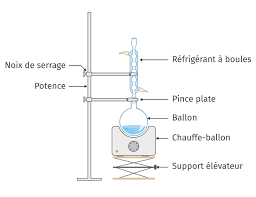
\includegraphics[width=\linewidth]{Ressources/montagereflux.png}
    \end{center}
\end{minipage}
\begin{minipage}{.6\linewidth}
    \caption{\textbf{Protocole}}
    \begin{itemize}
        \item Dans un ballon sec, introduite \SI{10,0}{mL} d'alcool benzylique et le volume d'acide éthanoïque indiqué dans le tableau du Doc. 2.
        \item Dans le ballon, ajouter dix gouttes d'acide sulfurique concentré et quelques grains de pierre ponce.
        \item Adapter le réfrigérant à eau au ballon, puis chauffer le mélange à ébullition douce pendant 25 minutes environ et arrêter le chauffage. L'état d'équilibre est considéré comme atteint au bout de 25 minutes.
        \item Quand le reflux a cessé, ajouter dans le ballon \SI{200}{mL} d'eau glacée et agiter le mélange.
        \item  Prélever un échantillon du milieu réactionnel dont le volume vous est indiqué par le professeur.
        \item Procéder alors au titrage de l'acide éthanoïque restant, dans le prélèvement.
    \end{itemize}
\end{minipage}

\textbf{Le réfrigérant :}\\
Le chauffage réalisé entraîne la formation de vapeurs. le réfrigérant va concenser ces vapeurs et les faire tomber dans le mélange.\\
Il n'y a donc \textbf{pas de perte de matière} et on peut ainsi faire réagir les réactifs plus longtemps, ce qui permet d'augmenter le rendement.\\

\textbf{Le système d'élévateur :}\\
Il permet l'arrêt du chauffage lorsque l'on baisse le chauffe-ballon en évitant tout risque de contact brûlant entre la main et le ballon.
\end{figure}

\begin{figure}[h!]
    \label{doc2}
    \caption{\textbf{Composition des mélanges réactionnels et résultats obtenus}}
    %\label{doc3}
    %Remarque : le volume titré tient compte de l'ajout de \SI{200}{mL} d'eau distillée glacée.\\
    \begin{tabular}{|>{\centering}m{.6\linewidth}|>{\centering}m{.1\linewidth}|>{\centering}m{.1\linewidth}|>{\centering\arraybackslash}m{.1\linewidth}|} \hline
    \textbf{Mélange} & \textbf{1} & \textbf{2} & \textbf{3}\\
    \hline
    Volume d'alcool benzylique (mL) & \num{10,0} & \num{10,0}  &\num{10,0} \\
    \hline
    Quantité initiale d'alcool benzylique $n(alcool)_i$ & & & \\
    \hline
    Volume d'acide éthanoïque (mL) & \num{5,5} & \num{11,0} & \num{55,0}\\
    \hline 
    Quantité initiale d'acide éthanoïque $n(AH)_i$ & & & \\
    \hline
    Volume titré $V_{titre}$ (mL) & \num{20,0} & \num{10,0} & \num{1,0}\\
    \hline
    Volume de soude versée à l'équilibre $V_E$ (mL) & & & \\
    \hline
    Quantité d'acide titré $n(AH)_{titre}$ (mmol) & & & \\
    \hline
    Coefficient multiplicateur & \num{10,8} & & \\
    \hline
    Quantité finale d'acide éthanoïque dans le mélange réactionnel $n(AH)_f$ (mmol) & & & \\
    \hline
    Quantité finale d'ester $n(ester)_f$ (mmol) & & & \\
    \hline Quantité maximale d'ester $n(ester)_{max}$ (mmol) & & & \\
    \hline
    Rendement $\eta$ (\unit{\percent})& & &  \\
    \hline
    \end{tabular}
\end{figure}

\begin{figure}[h!]
    \label{doc3}
    \caption{Tableau d'avancement de la réaction de synthèse}
    \begin{tabular}{|>{\centering}m{.15\linewidth}|>{\centering}m{.15\linewidth}|>{\centering}m{.15\linewidth}|c|>{\centering}m{.15\linewidth}|>{\centering\arraybackslash}m{.15\linewidth}|}
    \hline
    &\multicolumn{2}{c|}{\textbf{\ce{alcool(l) + acide (l) }}} & \ce{<=>}&\multicolumn{2}{c|}{\ce{ester (l) + H2O(l)}}\\
    \hline
    %État du système & $n(alcool)$ & $n(AH)$ && $n(ester)$ & $n(eau)$\\
    %\hline
    Initial & $n(alcool)_i$ & $n(AH)_i$ && 0 & 0\\
    \hline
    $x$ &  &  &&  & \\
    \hline
    Final &  & &&  & \\
    \hline
    \end{tabular}
\end{figure}

\begin{figure}[h!]
    \caption{Le titrage colorimétrique}
    \begin{minipage}{0.4\linewidth}
    \begin{center}
        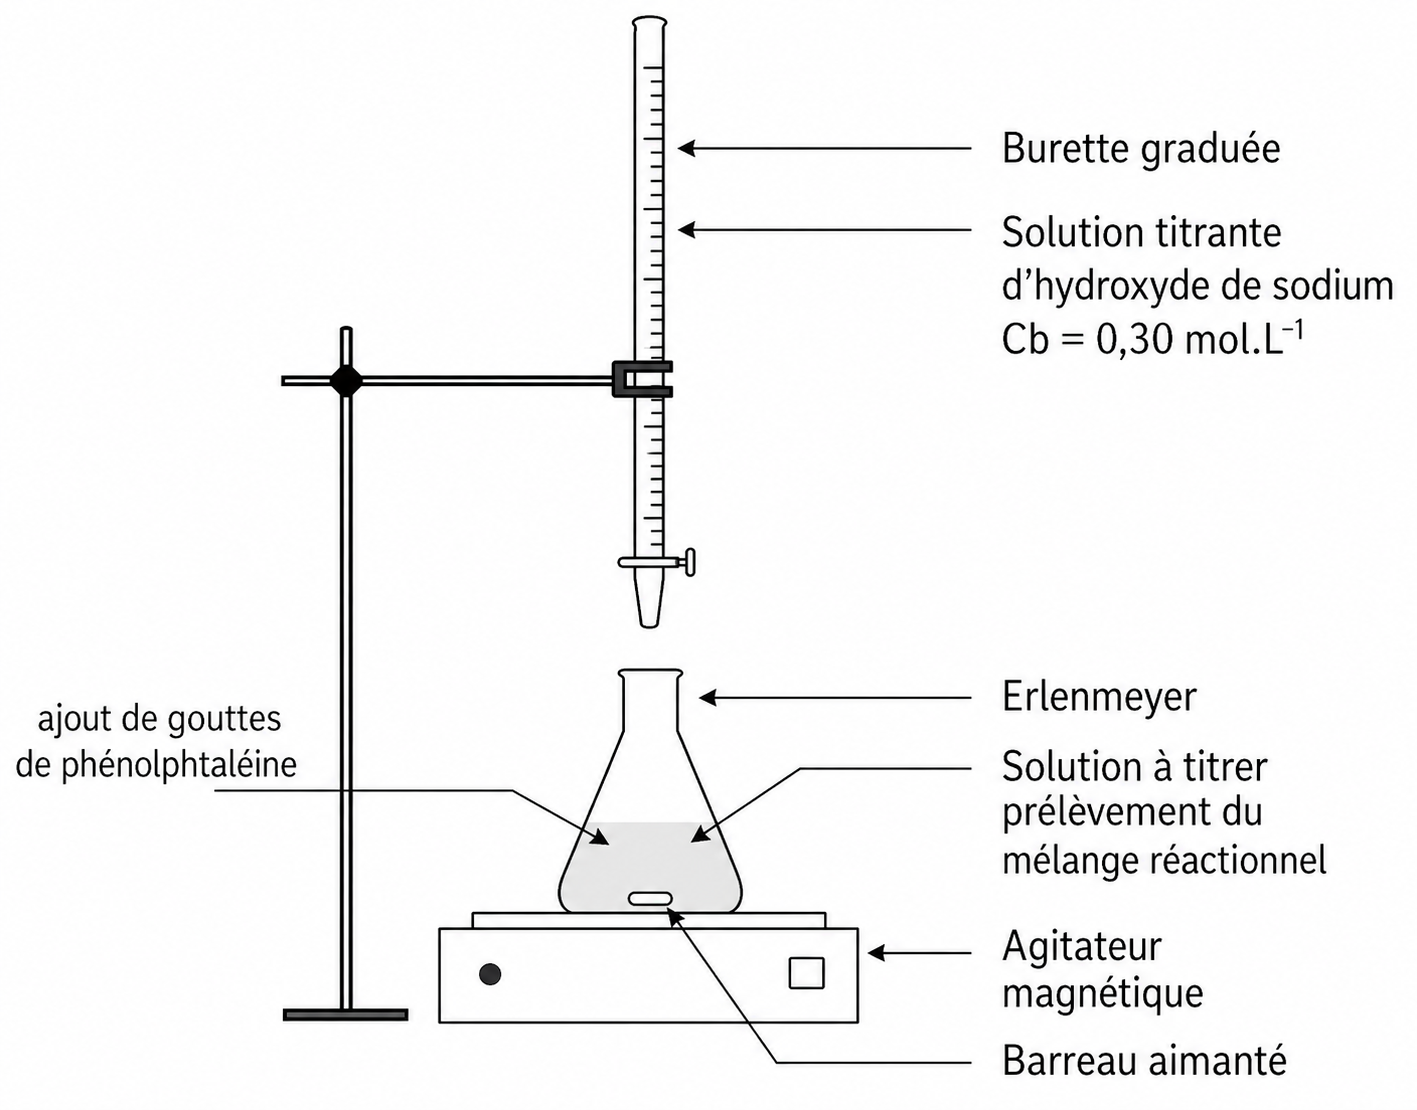
\includegraphics[width=\linewidth]{Ressources/ChatGPT Image 26 avr. 2026, 21_25_27.png}
    \end{center}
    \end{minipage}
    \begin{minipage}{0.5\linewidth}
    Il est nécessaire d'ajouter de l'eau distillée dans l'erlenmeyer pour avoir un volume suffisant.\\
    L'indicateur coloré de pH, la phénolphtaléine, est incolore en milieu acide et devient rose en milieu basique.\\
    \end{minipage}
    
\end{figure}

\textbf{Questions}\\
\begin{enumerate}
    \item Réecrire l'équation de la réaction de synthèse avec les formules semi-développées.
    \item Compléter le tableau d'avancement de la réaction de synthèse.
    \item Déterminer les quantités initiales de réactifs et les quantités maximales d'ester synthétisé et compléter les lignes correspondantes du tableau du Doc. 3.
    \item Expliquer le rôle du titrage réalisé lorsque la synthèse est terminée.
    \item Déterminer l'équation de la réaction de titrage réalisée et en déduire l'expression de la quantité d'acide titré.
    \item La quantité d'acide éthanoïque présenté à l'état final dans le mélange 1 peut être obtenue par le calcul : $$n(AH)_f = 10,8\times n(AH)_{titre}$$ Justifier ce calcul et en déduire les autres coefficients multiplicateurs.
    \item Exprimer la quantité d'ester finale en fonction des quantités $n(AH)_i$ et $n(AH)_f$.
\end{enumerate}
\textbf{Exploitation des résultats}\\
\begin{enumerate}[resume]
    \item Compléter le tableau à l'aide de vos résultats et ceux des autres binômes.
    \item Que peut-on conclure sur les rendements obtenus ?
\end{enumerate}
\end{document}